\subsubsection{Eliminaci\'on Gaussiana vs Factorizaci\'on de Cholesky (modificaci\'on del t\'ermino independiente)}
\textbf{Hip\'otesis:} El algoritmo de Eliminaci\'on Gaussiana tiene complejidad $O(n^{3})$ mientras que el algoritmo de Factorizaci\'on de Cholesky tiene complejidad $O(n^{2})$ para recalcular las soluciones de los sistemas por modificaciones en el t\'ermino independiente. \\

Dado que Gauss modifica el t\'ermino independiente en cada iteraci\'on para alcanzar el sistema equivalente, modificarlo posteriormente implica volver a cargar los datos iniciales y a aplicar la Eliminaci\'on para resolverlo con el nuevo b.

En el caso de Cholesky, no se hace uso del t\'ermino independiente, por lo tanto basta calcular una \'unica vez la factorizaci\'on y resolver el sistema para cada b que se quiera.

Para verificar esto, nuestra implementaci\'on verifica que las soluciones de cada algoritmo sean las mismas para cada b. Esta igualdad se realiza con un determinado grado de tolerancia debido a la aritm\'etica de punto flotante.

Una vez que determinada la igualdad de las soluciones, procedemos a analizar el costo de cada m\'etodo. Corrimos el algoritmo con instancias de 50 a 500 equipos con intervalos de 50 y trabajamos con 20 modificaciones de t\'ermino independiente, sin modificar la matriz de Colley inicial.

\begin{figure}[h!]
  \begin{center}
	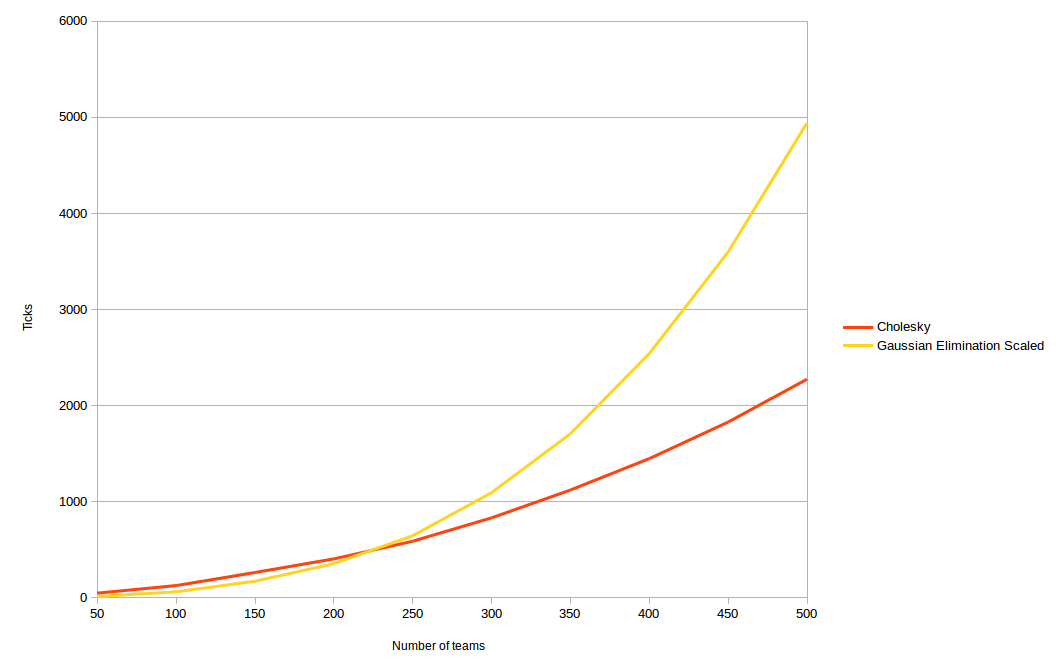
\includegraphics[scale=0.50]{imagenes/cuantitative/bChange/ColleyMatrixCuantitativeBChangeAnalysis.png}
	\caption{Comparaci\'on de complejidad temporal modificando el b en cada iteraci\'on}
	\label{bChange}
  \end{center}
\end{figure}

Este gr\'afico tiene la curva de la Eliminaci\'on Gaussiana escalada para poder visualizarlo en conjunto con la otra.

Puede apreciarse que el m\'etodo de Gauss tiene una curva mucho m\'as pronunciada que la factorizaci\'on y se parecen a las de las complejidaded esperadas. No obstante no podemos discernir si son la misma pero multiplicadas por una constante, de modo que el p\'roximo paso es suavizarlas.

\begin{figure}[h!]
  \begin{center}
	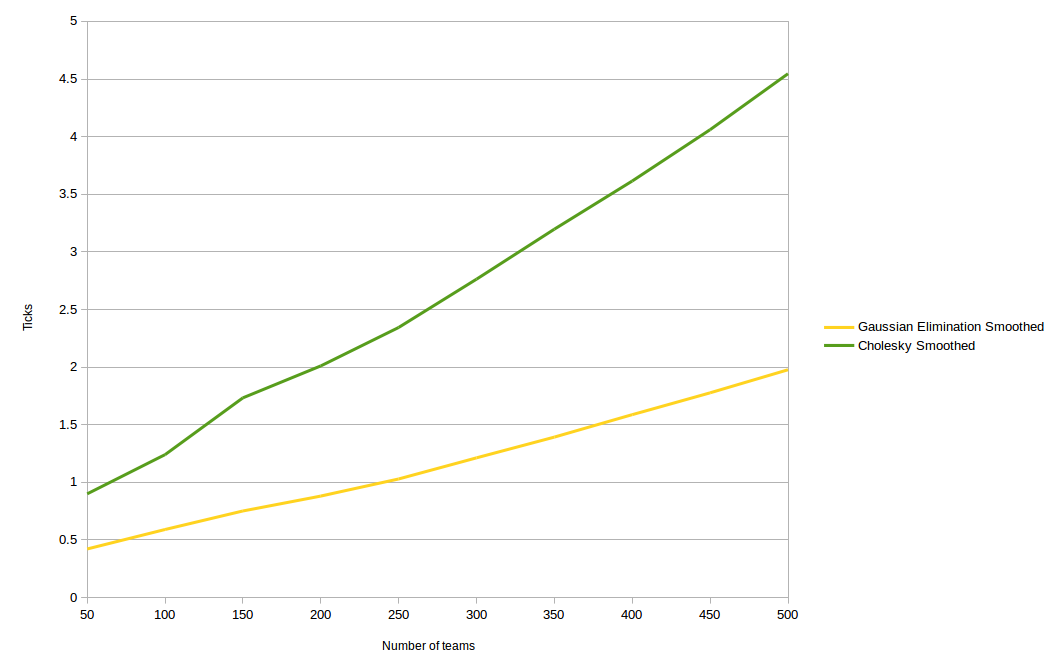
\includegraphics[scale=0.50]{imagenes/cuantitative/bChange/ColleyMatrixCuantitativeBChangeAnalysisSmoothed.png}
	\caption{Comparaci\'on de complejidad temporal modificando el b en cada iteraci\'on suavizado}
	\label{bChangeMoreSmoothed}
  \end{center}
\end{figure}

\newpage

La curva de Gauss fue dividida por el cuadrado del tama\~no de la entrada, mientras que Cholesky fue dividivo por el tama\~no de la entrada. Ambas se ven lineales, de modo que podr\'iamos pensar que la hip\'otesis es correcta. No obstante, vamos a dividir nuevamente a cada curva por el tama\~no de la entrada y ver si la resultante se parece a una funci\'on constante.

\begin{figure}[h!]
  \begin{center}
	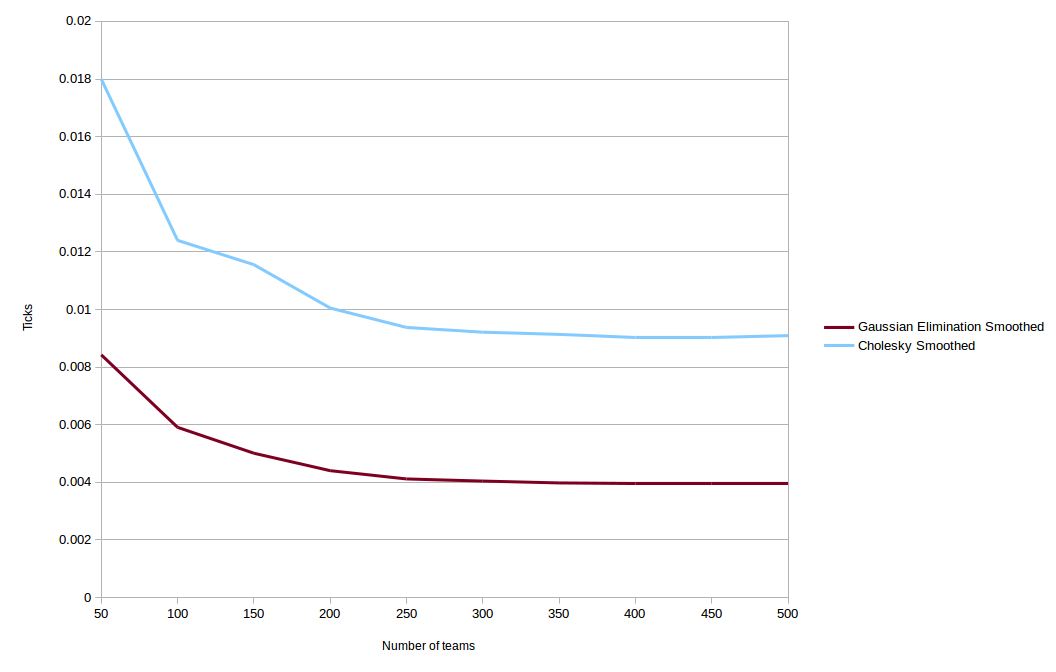
\includegraphics[scale=0.50]{imagenes/cuantitative/bChange/ColleyMatrixCuantitativeBChangeAnalysisConstant.png}
	\caption{Comparaci\'on de complejidad temporal modificando el b en cada iteraci\'on suavizado}
	\label{bChangeSmoothed}
  \end{center}
\end{figure}

Efectivamente, a partir de muestras de tama\~no 250 se aprecia que ambos algoritmos tienden a una constante. Las instancias de n peque\~nos tienen una cantidad de ticks levemente mayor pero, esto es atribuible a motivos de cach\'e del procesador y procesos paralelos.
